
\documentclass{template/openetcs_article}
% Use the option "nocc" if the document is not licensed under Creative Commons
%\documentclass[nocc]{template/openetcs_article}
\usepackage{lipsum,url,color}
\usepackage{tikz}
\usetikzlibrary{calc}
\usepackage{listings}

\graphicspath{{./template/}{.}{./images/}}
\begin{document}
\frontmatter
\project{openETCS}

%Please do not change anything above this line
%============================
% The document metadata is defined below

%assign a report number here
\reportnum{OETCS}

%define your workpackage here
\wp{Work-Package 7: ``Toolchain''}


\author{Roberto Kretschmer, Stefan Rieger}

\affiliation{TWT GmbH Science and Innovation\\
Bernh\"auser Stra\ss e 40-42\\
73765 Neuhausen}

\title{Model evaluation report: SystemC model of UNISIG Subset-026-3 3.5 Management of Radio Communication (MoRC)}

% define the coverart
\coverart[width=350pt]{openETCS_EUPL}

\reporttype{Model Description}

%\begin{document}

\maketitle
\tableofcontents
\listoffiguresandtables
\newpage

\section{Short Introduction to Formalism and Tool}
\label{sec:short-intr-form}

SystemC is a C++ library providing an event-driven simulation interface suitable for electronic system level design. It enables a system designer to simulate concurrent processes. SystemC processes can communicate in a simulated real-time environment, using channels of different data types (all C++ types and user defined types are supported). SystemC supports hardware and software synthesis (with the corresponding tools). SystemC models are executable.

\subsection{SystemC Evaluation Models for WP7}

Within the context of Work Package 7 we are working on two different models:
\begin{itemize}
  \item A SystemC model for Subset 026, Section 3.5, ``Radio Communication'' which is currently developed by TWT
  \item A SystemC model regarding the braking curves in Subset 026. This model is being developed by the University of Rostock
\end{itemize}

At the moment (\today), the models are still in an incomplete state but at least a basic version of the radio communication model is ready for assessment. We will provide updates in alignment with the review process as soon as we are able to integrate additional features. As the scope of WP7 is \emph{not} to provide a complete system model, we believe that also incomplete models are suitable to get an idea of the modeling language and judge its suitability for application within the project.

\paragraph{Purpose of this Documentation}

This documentation shall give a short introduction to SystemC, to our modeling process, which is based on a top-down approach based on SysML and code generation thereof, and the structure of our models.

\subsection{Basic Concepts of SystemC}

A SystemC model is constructed of so-called \emph{modules}, C++ classes derived from a common base class \verb|sc_module|. Modules may be nested and are interconnected by \emph{channels}. There is a variety of different pre-defined channels, such as signal-channels (behavior as a shared variable or a hardware wire) or FIFO-queues. In addition, it is possible to define custom, complex channels. Modules usually contain \emph{threads} and \emph{event-triggered methods} that are executed in parallel. Threads and methods may register/wait for certain events in the system, such as the transmission of a message via a channel or a value change of a signal.

\subsubsection{Defining Modules, Ports and Channels}


\newcommand{\tikzrect}[1]{\draw ($#1+(-0.25,-0.25)$) -- ($#1+(-0.25,+0.25)$) -- ($#1+(+0.25,+0.25)$) -- ($#1+(+0.25,-0.25)$) --cycle;}
\newcommand{\tikzport}[4]{\draw[fill=white] ($#1+(-0.25,-0.25)$) -- ($#1+(-0.25,+0.25)$) -- ($#1+(+0.25,+0.25)$) -- ($#1+(+0.25,-0.25)$) --cycle;
                          \draw[arrows=#2] ($#1+(-0.15,0)$) -- ($#1+(+0.15,0)$);
                          \path ($#1+#3$) node {#4};}

\begin{figure}
\begin{center}
\begin{tikzpicture}
\draw (0,2) -- (2,2) -- (2,0) -- (0,0) --cycle;
\path (1,1.5) node {Module A};
\draw (-1,4) -- (4,4) -- (4,-1) -- (-1,-1) --cycle;
\path (1.5,3.5) node {Module B};
\draw (8,-1) -- (8,4) -- (11,4) -- (11,-1) --cycle;
\path (9,3.5) node {Module C};
\tikzport{(4,2.5)}{->}{(-0.75,0)}{Port1}
\tikzport{(4,0.5)}{<-}{(-0.75,0)}{Port2}
\tikzport{(8,2.5)}{->}{(+0.75,0)}{Port3}
\tikzport{(8,0.5)}{<-}{(+0.75,0)}{Port4}

\foreach \x in {5.0,5.5,6.0,6.5,7.0} {
   \tikzrect{(\x,2.5)}
}

\draw (4.25,2.5) -- (4.75,2.5);
\draw (7.25,2.5) -- (7.75,2.5);
\path (6,3) node {FIFO channel};

\draw (4.25,0.5) -- (7.75,0.5);
\path (6,1) node {signal channel};
\end{tikzpicture}
\end{center}

\caption{Interconnected SystemC Modules}
\label{fig:modulestructure}
\end{figure}

Figure~\ref{fig:modulestructure} depicts a simple example structure of a SystemC model. Here we have three modules, where Module A is a sub-module of Module B. Modules B and C are interconnected with two channels. The upper one is a FIFO queue providing a buffered message channel, whereas the lower connection is realized by a signal channel transmitting data directly. For connecting channels, modules provide \emph{ports}. Ports are pre-defined interfaces supporting, e.g., reading or writing operations. Ports are often directed, i.e., there are input and output ports.

To realize the structure from Figure~\ref{fig:modulestructure} we could declare the modules as follows:

\lstset{language=C++, numbers=left, numberstyle=\tiny,showstringspaces=false} 
{\small
\begin{lstlisting}
SC_MODULE(ModuleA){
   ...
};

SC_MODULE(ModuleB){
   sc_port<sc_fifo_out_if<int> > port1;
   sc_port<sc_signal_in_if<int> > port2;

   ModuleA subsystem;
   ...

};

SC_MODULE(ModuleC){
   sc_port<sc_fifo_in_if<int> > port3;
   sc_port<sc_signal_inout_if<int> > port4;
   ...
};
\end{lstlisting}
}

As you can see, the ports are declared with the corresponding type (in this case \verb|sc_fifo_out_if|, \verb|sc_fifo_in_if|, \verb|sc_signal_in_if|, and \verb|sc_signal_inout_if|\footnote{Note that SystemC does not provide an interface that only allows writing to and not reading from signal channels. This makes sense as a read has no effect on the state of the channel (in contrary to FIFO channels). Alternatively one could use \texttt{sc\_out<int>} instead of \texttt{sc\_port<sc\_signal\_inout\_if<int> >}. We use the latter to get a unified notation for ports and to simplify code generation from, e.g., SysML.}) which are interfaces to the corresponding channels and specified as C++ template parameter. In this example all interfaces have been set up for the message/signal type \verb|int|\footnote{Note that it is necessary to specify a type here. Of course, also custom types may be used.}.

\subsubsection{Connecting the Modules}
Although we have defined all three modules, the interconnections are not defined yet as no module has been instantiated and the connections between the modules have not been established by providing the corresponding channels. This could be done as follows in the \verb|sc_main| function:

{\small
\begin{lstlisting}
int sc_main(int argc, char* argv[]) {
   ...
   // Instantiate modules
   ModuleB b("ModuleB instance");
   ModuleC c("ModuleC instance");

   // Instantiate channels
   sc_fifo<int> fifo;
   sc_signal<int> signal;

   // Bind ports to channels
   b.port1(fifo);
   c.port3(fifo);
   b.port2(signal);
   c.port4(signal);
   ...
}
\end{lstlisting}
}

\subsubsection{Writing to and Reading from Ports and Channels}

There is no unified way to access ports or channels as they may be intended for different purposes. E.g, where for a signal a single value suffices one could define a channel type that includes addressing and payload to simulate network protocols. For the predefined channels, such as \verb|sc_signal| and \verb|sc_fifo| methods \verb|write| and \verb|read| are supported to write values to and read values from a channel/port, respectively. The semantics in those cases, however, is different:

While for \verb|sc_signal| writes and reads are executed immediately and do not have any precondition, writes to and reads from \verb|sc_fifo| are blocking if the buffer is full on write or no data is available on read. However, there are also non-blocking versions (\verb|nb_write| and \verb|nb_read|) that terminate immediately and a return value may be used to determine whether actually any data was written/read.

Thus, in our example write or read operations could look as follows:
{\small
\begin{lstlisting}
// In sc_main using the channels:

fifo.write(1);            // blocks if FIFO buffer is full
int x = signal.read();    // returns immediately

...

// In Module 3 using ports:

while(true) {             // reads from FIFO ports are often executed
                          // in a loop as the operation is blocking
   ...
   int x = port3->read(); // blocks until data is available
  ...

}
...
port4->write(0);          // Non-blocking write to a signal port
...
\end{lstlisting}
}

In the above code listing it is evident that the access to the ports from the modules is preceded by the \verb|->| operator. This is not necessary when directly writing to the channels.

\subsubsection{Threads and Event-Triggered Methods}

SystemC make heavy use of concurrency and employs an event-based architecture. Events, such as the change of a signal value, can trigger actions. SystemC provides two concepts for this, both of which are realized as member functions within a SystemC module:

\begin{description}
\item[Threads] (\verb|SC_THREAD|) are versatile processes that can be halted at any moment and any number of times during their execution by using a \verb|wait| statement. A thread is run only once. Often, a thread is meant to run for the whole duration of the simulation. This can be achieved by using an infinite loop. A thread can be suspended for a certain amount of time or until an event occurs. The events that a thread is sensitive to are not necessarily statically defined.
\item[Methods] (\verb|SC_METHOD|) will run more than once when they are triggered by an event and cannot be suspended during their execution. In addition, they usually have a static sensitivity list.
\end{description}

Let us look again at our example. In Module C we could define a thread that waits for an incoming integer on Port 3 (FIFO channel) and then writes it out to Port 4 (signal channel). This can be done as follows:

{\small
\begin{lstlisting}
SC_MODULE(ModuleC){
   sc_port<sc_fifo_in_if<int> > port3;
   sc_port<sc_signal_inout_if<int> > port4;
   ...

   void mythread(){
      while(true){
         int x = port3->read();   // Read from FIFO
         cout << "Read value " << x << " from Port 3 \n";
         port4->write(x);         // Write to signal
      }
   }  

   // Module constructor, here by using the default macro; can
   // also be defined manually if additional parameters are necessary
   SC_CTOR(ModuleC){
      SC_THREAD(mythread);  // Thread initialization
   }
};
\end{lstlisting}
}

Equivalently, one could also use the non-blocking read of the FIFO and explicitly use the \verb|wait| statement:

{\small
\begin{lstlisting}
   void mythread(){
      while(true){
         wait(port3->data_written_event()); 
         int x;
         port3->nbread(x);  //Non-blocking read
         cout << "Read value " << x << " from Port 3 \n";
         port4->write(x);
      }
   }  
};
\end{lstlisting}
}

In Module B we possibly want to output the state of the signal connected to Port 2 when its value changes. This can be accomplished as follows:

{\small
\begin{lstlisting}
SC_MODULE(ModuleB){
   sc_port<sc_fifo_out_if<int> > port1;
   sc_port<sc_signal_in_if<int> > port2;
   ...

   void print_change(){
     cout << "Port 2 value changed to " << port2->read() << endl;
   }

   SC_CTOR(ModuleB){
      SC_METHOD(print_change);  // Initialize event-triggered method
      sensitive << port2;       // Make method sensitive to events on port2
   }

};
\end{lstlisting}
}

Thus, whenever the signal connected to Port 2 changes its value, the method \verb|print_change| is called. Please note, that in our model of the ETCS radio communication setup we do not use \verb|SC_METHOD|s for a more streamlined approach. Everything that can be done with \verb|SC_METHOD|s can be also done with \verb|SC_THREAD|s.

\subsubsection{The SystemC Simulation Scheduler}

Here we will later-on add some information about the SystemC simulation scheduler.


\section{Modeling Strategy}
\label{sec:modeling-strategy}

\subsection{Modeling Strategy: SysML}

In the following we shortly introduce the basic modeling strategy, which is based on the decision to use SysML as high level modeling language.
In line with the openETCS proposal we developed a modeling workflow of radio communication (MoRC) based on Subset 026, Section 3.5, ``Radio Communication'' of the ETCS standard following a model driven approach, which is based on available open source tools.
The main goal of this approach is a step-wise refinement of models of the SUT to executable code.
One obvious question in this regards is what underlying engineering process one chooses, i.e. which steps or abstractions levels are suitable for the development of the SUT.
On the one hand SystemC allows the definition of system level descriptions on TLM level which can later be enhanced with further details or the selection of a certain Model of Computation respectively. 
On the other hand even at the TLM level SystemC might be regarded as too detailed for early stages of system development.
Here one is rather interested in high level modeling languages such as UML or SysML which are well suited for the overall system concept and for easy communication with stakeholders of diverse expertise.
However there is a semantical gap between these high level modeling languages and the executable code.
In the literature different approaches are suggested to bridge this gap between UML/SysML and SystemC.
These are mainly realized by defining UML profiles to extend SysML by introducing stereotypes that represent SystemC constructs, e.g., \cite{Mueller2011,Riccobene2012}.
In our approach we describe use the standard SysML stereotypes to model the MoRC and infer automatically a TLM description in SystemC using code generation.
One advantage is that the modeler is not required to learn new language elements.
However, since the code generation fixes the semantics of a given SysML model element to a certain SystemC construct the modeler needs to have a basic understanding of this mapping in order to achieve the intended result.\\

\subsubsection{Structural modeling}

SysML is models consist of structural and behavior elements. In our workflow we first created a top level block diagram. Blocks represent the fundamental structural unit of the SysML model. To create the SysML model we use the Eclipse modeling framework (Indigo version) with activated Papyrus plug in. Papyrus doesn't support the newest version of SysML 1.3, i.e. full and proxy ports are not defined instead we have used flow ports, which is sufficient for our needs. An example of the Eclipse user interface with activated papyrus perspective is shown in Figure~\ref{fig:eclipseIDE}.

\begin{figure}
\begin{center}
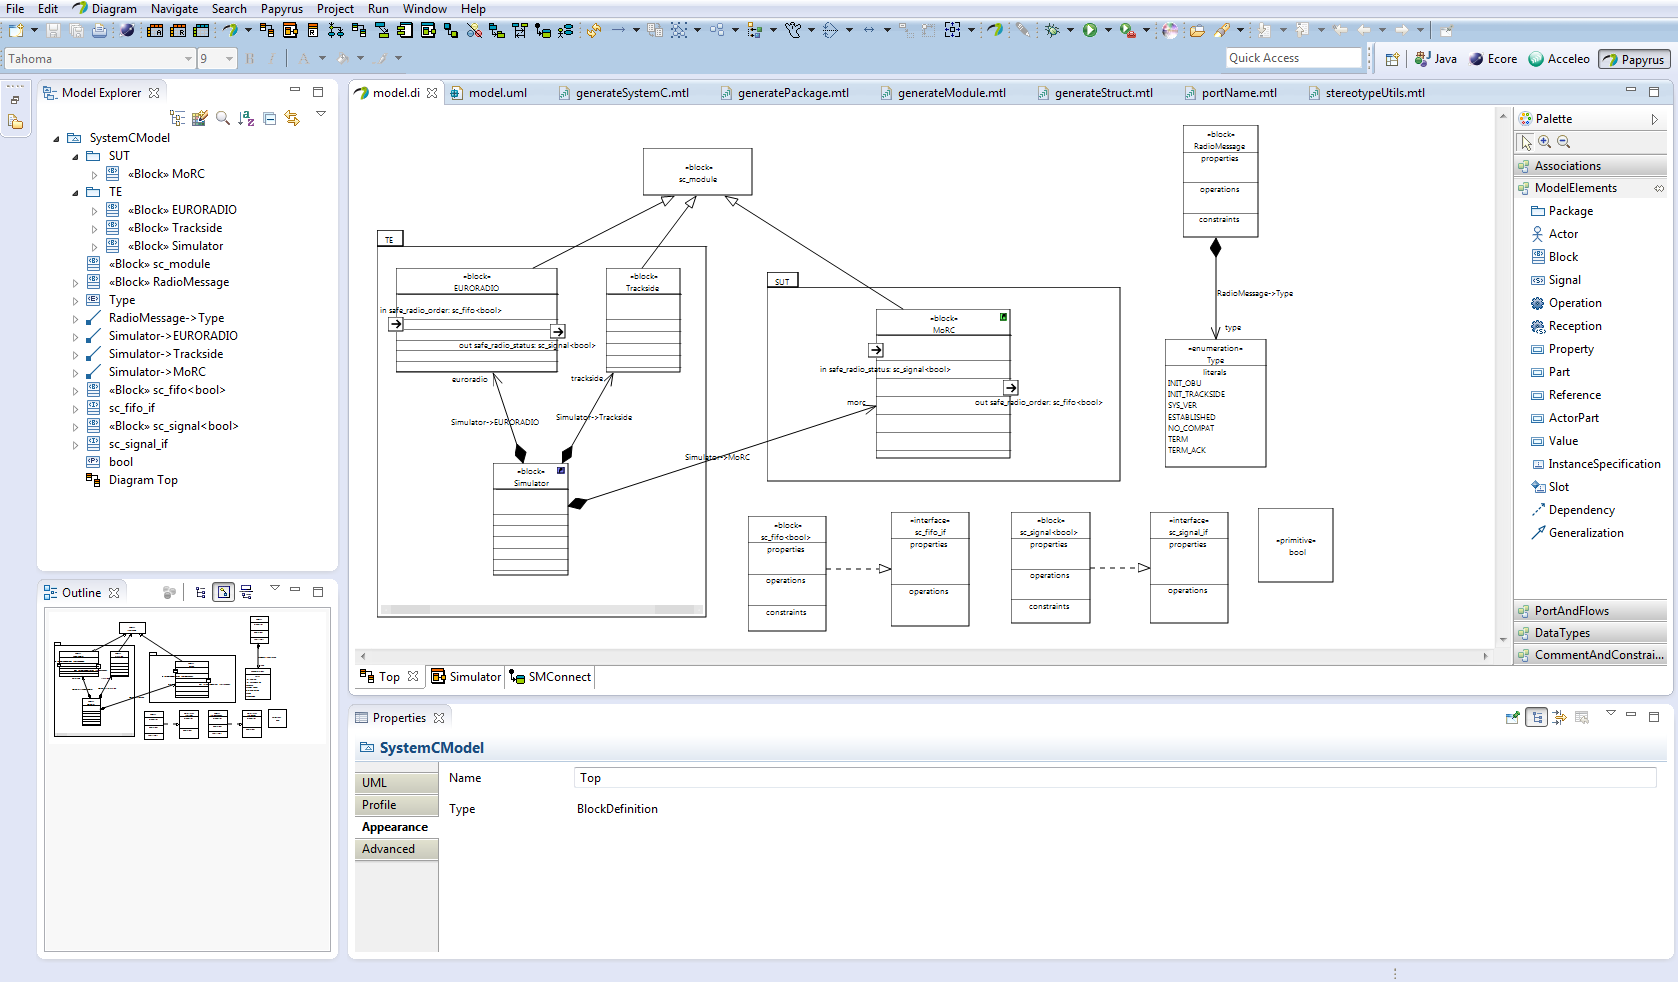
\includegraphics[scale=0.3]{figures/papyrus_screenshot}
\end{center}
\caption{Eclipse IDE with enabled Papyrus plugin, showing the SUT SysML model.}
\label{fig:eclipseIDE}
\end{figure}

Figure~\ref{fig:sysmlToplevel} shows the top level block diagram. This diagram also shows two packages, which are embedded in the top level package, which is called \verb SystemCModel. The two nested packages are "`TE"' for the test environment and the SUT package, which contains the actual MoRC model. The use of package allows for a better organization of the overall model and are later mapped to different SystemC namespaces (see below). This way the test environment is clearly separated from all the SUT parts. The TE is needed in order to model how the SUT can be stimulated and eventually simulate it's behavior with the SystemC runtime environment. To distinguish blocks that form the SystemC modules from other block, e.g. primitive and complex data types, we introduced the block  \verb sc_module and create links of type "`Generalization"' (c.f. Fig.~\ref{fig:sysmlToplevel}). The other blocks are "`RadioMessage"' which is a data type containing of the type of the message and type and interface definitions. The latter are used to specify, i.e. type the flow ports. 

\begin{figure}
\begin{center}
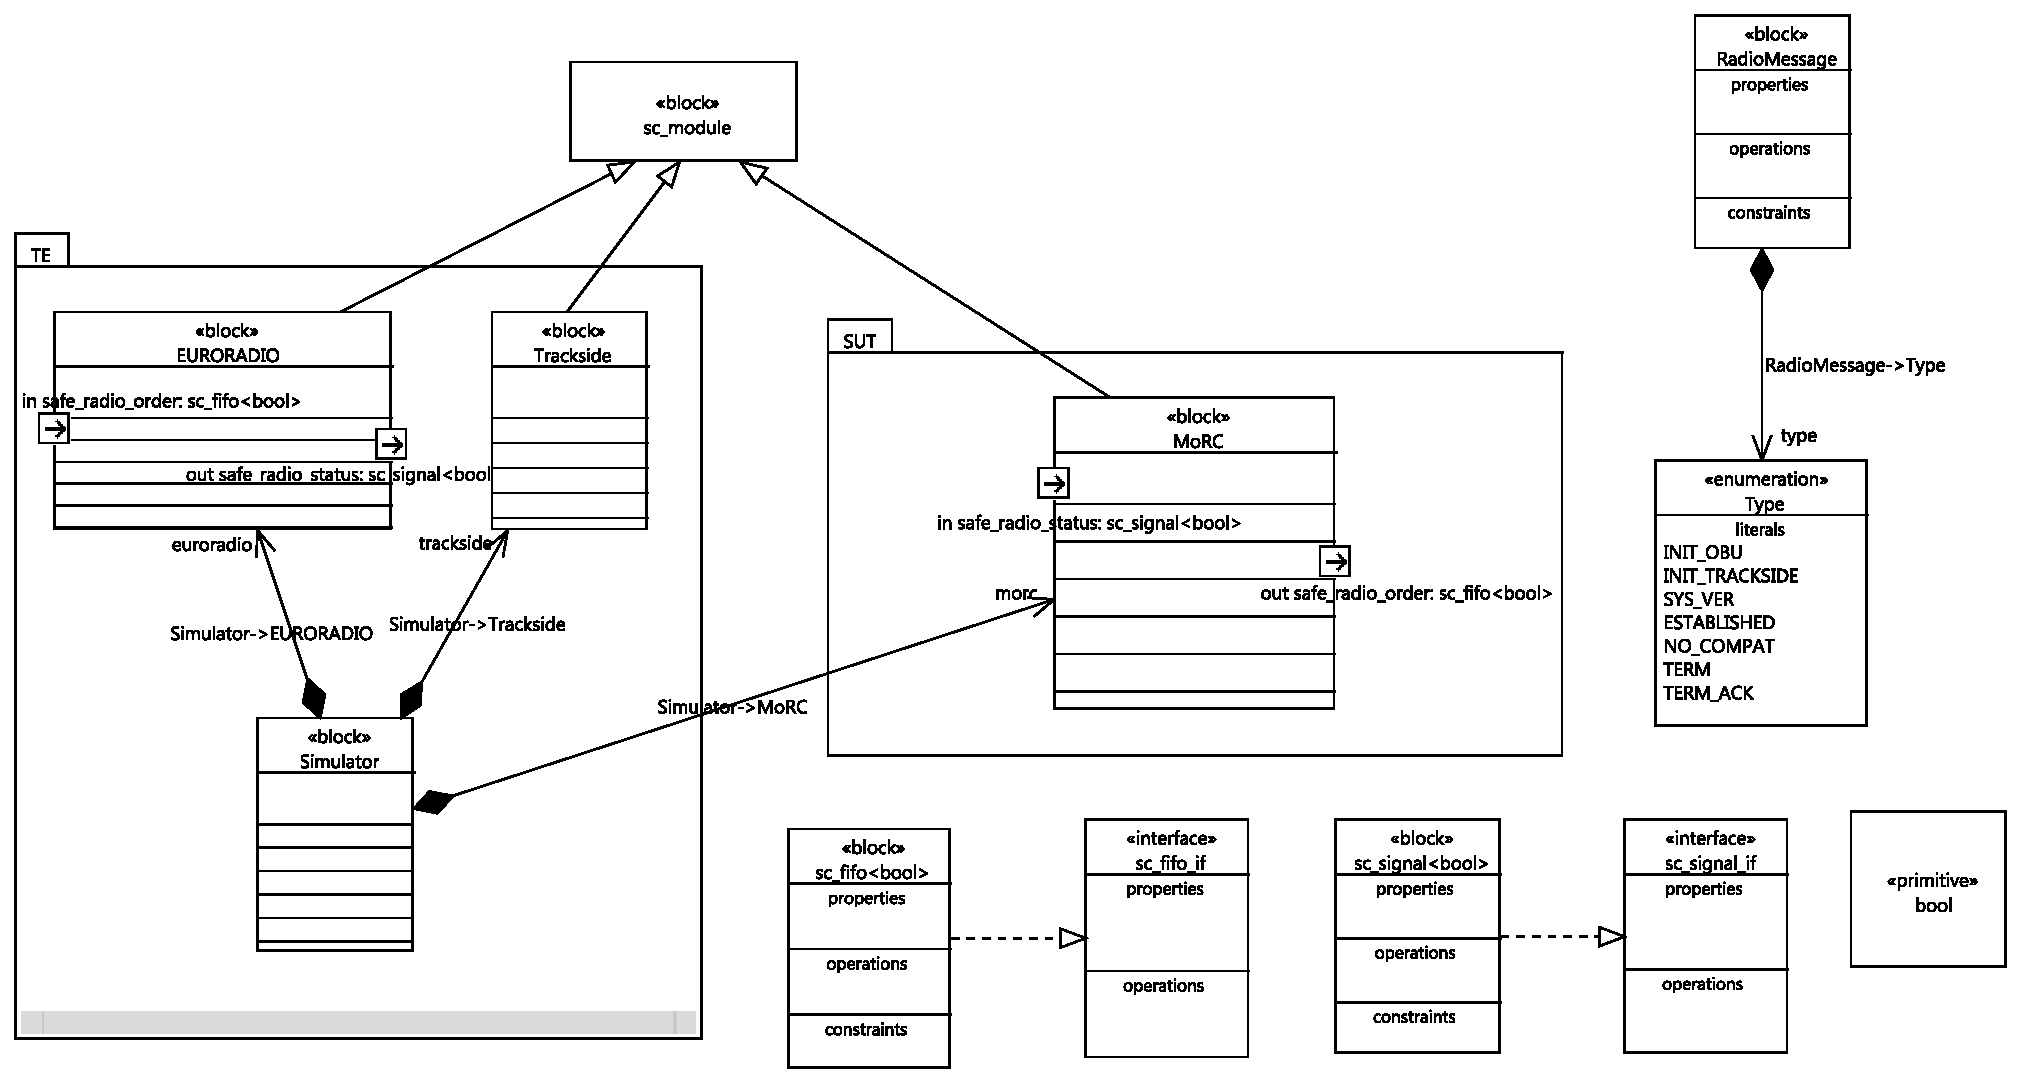
\includegraphics[scale=0.4]{figures/Top}
\end{center}
\caption{Top level SysML block definition diagram.}
\label{fig:sysmlToplevel}
\end{figure}

The block \verb Simulator is the main part of the TE, which is used to connect the instances of the modules and describe the behavior of the TE. At this point we use this block to model the interconnection of the MoRC to the EURORADIO and Trackside model components shown in the internal block definition diagram in Figure~\ref{fig:simulatorIbd}. Note that this block itself is not derived from \verb sc_module, i.e. it is not a SystemC module. The connectors in the internal block definition diagram shows the connection between the ports of the modules that were defined in the top level block diagram. Arrows in the flow ports indicate the direction of the data/signal flow, which can be either in, out, and inout. The type of the port shows the kind of data that is transmitted and the kind of connection: buffer, direct, fifo etc. In this case we connect the ports \verb safe_radio_status with a signal and a simple Boolean value is transmitted. For the \verb safe_radio_order we used a FIFO connection instead, which better captures the subset 26 requirements.

\begin{figure}
\begin{center}
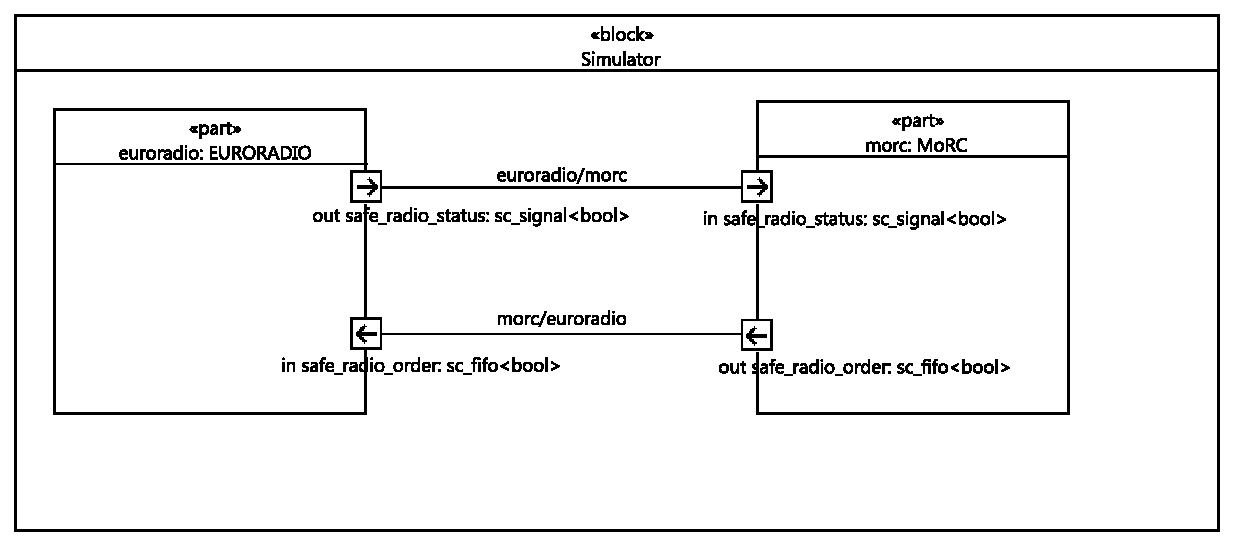
\includegraphics[scale=0.5]{figures/Simulator}
\end{center}
\caption{Example of the internal block diagram of the simulator.}
\label{fig:simulatorIbd}
\end{figure}

To realize the port types we introduce SystemC specific data types via interface and data type blocks (c.f. lower right part in Fig.~\ref{fig:sysmlToplevel}). We added a redefinable template signature to each interface to be able to model the possibility to transmit different data types with the respective interface. The blocks realizing the interfaces (dashed line with arrow in Fig.~\ref{fig:sysmlToplevel}) define a template binding assigning the template to the "`bool"' primitive. This template information is not shown in the block diagram and we had to use the model tree editor to realize these links, which is shown in Figure~\ref{fig:eclipseTemplates}. The redefinable template signature includes defines a formal classifier template parameter which is substituted withe actual primitive type \verb bool. These described characteristic SystemC model elements might later be added to a dedicated package for easy reuse in other SysML models.

%According to MDA methodology we have chosen to start with a generic SysML model that captures the general structure and behavior of the SUT.
%The model is shown in Figure.
%Papers 
%Starting 
%SysML has an ambiguous definition of the semantic. Thus we can use SystemC to define a certain semantic.
%Here we map SysML to SystemC language constructs.
%The mapping is shown in Table.

\subsubsection{Behavioral modeling}

SysML state machine are expecially suitable to model the SystemC event-based behavior.
The behavior of the MoRC is modeled with a state machine diagram, which we we will describe here in a upcoming version of this document.
The Acceleo-Eclipse plugin supports syntax hihlighting and code completion for the thus the coding is very convenient.
Further features comprise debugging...

\begin{figure}
\begin{center}
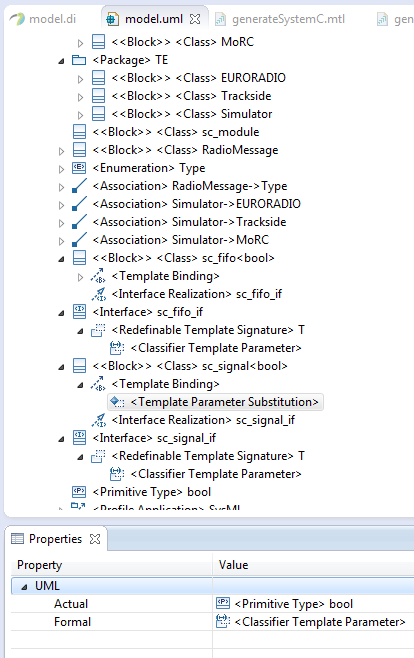
\includegraphics[scale=1]{figures/template_binding}
\end{center}
\caption{Using the Eclipse model editor to create UML template signatures and bindings}
\label{fig:eclipseTemplates}
\end{figure}

\subsection{Modeling Strategy: Code Synthesis}
%KRE:
%EMF, GMF, ACCELEO

In this section we describe the code generation of the SysML model using the Eclipse framework and the Acceleo Plugin.
In Eclipse our workflow is organized with two projects. The first, a Papyrus project, contains the the SysML model and the second is an Acceleo project that defines the SystemC code generation. The Acceleo plugin implements the MOF Model To Text Transformation Language (MOFM2T). Using the language one can traverse and query the SysML model tree to access all model elements and their attributes. The SysML/SystemC mapping definition is organized in modules containing templates. These templates are assigned to model elements. The principle of the template is What You Code Is What You Get (WYCIWYG), i.e. all text in the template that is not a MOFM2T language element is put in the transformation output. The language elements contain fundamental control flow constructs, such as loops and if statements as well as variable assignments. In addition it is possible to create files and to extend a template functionality by calling external Java services. For each module we included the SysML and UML profiles, which is needed to declare all types we use in our SysML model. This is achieved by adding the respective URIs when creating a new Acceleo project. The project is linked to our SysML model in the project creation wizard as well.\\

For the moment our code generator is able to create the structure of the model. For each module a one header and one cpp files is generated. In addition a main.cpp file is created which contains the channel binding according to the SysML model specification. In later version of this document we will describe the translation in more detail and include the transformation of the SysML state machines.


\section{Model Overview}
\label{sec:model-overview}

\subsection{SystemC Model for Subset 026 Radio Communication (TWT)}

When creating the SystemC model for the radio communication section of Subset 026, the idea was to have one part representing the system under test (SUT) and one part for the test environment (TE) that provides inputs and evaluates outputs of the SUT. To this end, we defined two C++ \emph{namespaces}, \verb|SUT| and \verb|TE|, each of which may contain several SystemC modules. This lead to the following model structure:
\begin{itemize}
  \item namespace \verb|SUT|
    \begin{itemize}
      \item module \verb|MoRC|: The \textbf{M}odule \textbf{o}f \textbf{R}adio \textbf{C}ommunication represents the system under test. It receives connection orders from the outside and interacts with the \verb|EURORADIO| module. Includes a state machine \verb|SMConnect| that models the connection setup. ($\rightarrow$ morc.h, morc.cpp)
    \end{itemize}

  \item namespace \verb|TE|
    \begin{itemize}
      \item module \verb|EURORADIO|: Simulates the behavior of an EURORADIO module setting up the safe radio connection. Failures of safe radio are simulated with an exponential probability distribution. ($\rightarrow$ euroradio.h, euroradio.cpp)
      \item module \verb|Trackside|: Simulates the trackside (RBC or RIU). ($\rightarrow$ trackside.h, trackside.cpp)
    \end{itemize}
  \item Global namespace
    \begin{itemize}
      \item \verb|RadioMessage|: data structure for exchanging messages with the trackside; includes an enum for the message types required by Subset 026, overloaded trace and stream output operators are provided ($\rightarrow$ radiomessage.h, radiomessage.cpp)
      \item \verb|sc_main|: the program entry point that is used for instantiating all modules, setting up the environment and starting simulation ($\rightarrow$ main.cpp)
    \end{itemize}
\end{itemize}

For a more detailed description of the model please refer to Section~\ref{sct:radiocommdetailed}.

\subsection{SystemC Model for Braking Curves (URO)}

To be filled by Uni Rostock

\section{Model Benefits}
\label{sec:model-highlights}

%benefits from using this modeling formalism for the case study
%
%Model analyis with model checkers based on SysML model is possible.
%(Cite our paper) gave an overview of different methods to formalize SysML.
%Similarly to the SysML model to SystemC tranformation we have shown, a tranformation to a formal model language like timed automata is possible.
%For this we can define another set of Acceleo templates and use the resulting code to drive a model checker as for example UPPAAL.
%
%An advantage of using the Eclipse IDE together with Papyrus is the possibility to extend the IDE with aditional plugins.
%Flexible code generation is possible.
%EMF allows the definition of arbitray DSL with Ecore.
%From this graphical editors and code generators can be created.


\section{Detailed Model Description}
\label{sec:deta-model-descr}

\subsection{Technical Realization SysML}
%KRE 
SysML mit Eclipse, Interfaces, Templates

\subsection{Detailed Description of the SystemC Radio Communication Model (TWT)}
\label{sct:radiocommdetailed}

In the following we will give a more detailed description of each module of the radio communication model.

\subsubsection{MoRC}

The Module of Radio Communication (MoRC) represents represents the interface for communication of the ETCS onboard unit (OBU) with the trackside. In the model it is the system under test (SUT). Thus, the MoRC interacts with the EURORADIO module that is responsible for setting up a safe radio communication and via EURORADIO with the trackside. Orders for connection establishment can be triggered by several OBU components, such as the driver module interface (DMI) or the balise transmission module (BTM). In the our model we do not need to worry which component issues an order as they all come in at the same \emph{port}.

In the code we prefix input ports with the letter \verb|i| and output ports with the letter \verb|o|. The MoRC possesses the following ports:
\begin{description}
  \item[\tt i\_conn\_order] Boolean FIFO port that is used by MoRC-external components to trigger the establishment of a connection. If a 1 is received the MoRC will try to establish a connection (if not already established), if a 0 is received it terminates a connection (if applicable).
  \item[\tt o\_conn\_status] This is a Boolean signal port to indicate to MoRC-external components whether a radio connection has been established.
  \item[\tt o\_safe\_radio\_order] This Boolean FIFO output port is used to communicate with the EURORADIO subsystem. If a message with the content 1 is transmitted, the EURORADIO subsystem shall try to establish a safe radio connection. Upon a 0, a potentially active safe radio connection shall be terminated.
  \item[\tt i\_safe\_radio\_status] Analogous to \texttt{o\_conn\_status}, this signal port is to be used by an EURORADIO subsystem to indicate whether a safe radio connection is established. Upon the establishment of a safe radio connection by EURORADIO, the MoRC will try to connect to an RBC or RIU.
  \item[{\tt o\_trackside} {\rm and }{\tt i\_trackside}] FIFO ports for communicating with the trackside (RBC or RIU). These ports are used for sending and receiving messages of type \verb|RadioMessage| ($\rightarrow$ radio\_message.h).
\end{description}

In its current version the MoRC module has three threads:
\begin{description}
  \item[\tt order\_handler()] Upon receiving a connection order via port \texttt{i\_conn\_order} a state machine for setting up the radio connection is instantiated and given control. For more details regarding state machine modeling please refer to Section~\ref{sct:modellingsm}. Connection termination is not implemented yet.
  \item[\tt safe\_radio\_handler()] Listens on the port \texttt{i\_safe\_radio\_status} to detect the establishment or failure of a safe radio connection. Triggers the \emph{event} \verb|conn_lost_event| if the safe radio connection could not be reestablished within 5 minutes of simulation time.
  \item[\tt conn\_status\_signal\_driver()] This is a set that \emph{drives} the \texttt{o\_conn\_status} signal by listening for the events \verb|conn_established_event| and \verb|conn_lost_event|. Actually this thread is only necessary because in SystemC it is not allowed to write to a signal channel from multiple threads.
\end{description}


\subsubsection{Modelling State Machines}
\label{sct:modellingsm}

In our model the MoRC also contains a SystemC representation of a state machine that is used to model the connection setup. We found that this actually simplifies the control-flow and makes it more readable. In addition this method enables the transformation of SysML state charts to SystemC in a straightforward manner.

The transformation idea is quite simple: 
\begin{enumerate}
  \item Create a C++ function for every state in your state machine, in the following called \emph{state function}. In our model these have been prefixed with \verb|state_| and encaspulated in the subclass \verb|SMConnect|.
  \item Each state function may execute a certain actions and before it exits must fix the consecutive state to be executed. This is achieved by assigning to a function pointer the function representing the consecutive state (in our case this function pointer is \verb|SMConnect::next_state|). There may be several alternatives depending on the state of the system. If there is no consecutive state, \verb|NULL| is assigned.
  \item Call the function pointer in a loop until its value is \verb|NULL|. 
\end{enumerate}

\emph{Note:} You could achieve the same by introducing a \verb|switch| statement in the main loop and a \verb|case| for each state. But this is less clear in our opinion and increases the amount of code significantly.

The following code excerpt from our model illustrates this process\footnote{For more clarity we removed some debug outputs.}. It shows a state function for the case that a connection order has been received. If the connection status is 1 (connection is established) we are done and assign \verb|NULL| to \verb|next_state|, otherwise we move on to the next state function \verb|state_not_connected_connection_order()|.

{\small
\begin{lstlisting}
void MoRC::SMConnect::state_connection_order_received() {
    if (parent.o_conn_status->read())
        next_state = NULL;
    else 
	next_state = &SMConnect::state_not_connected_connection_order;
}
\end{lstlisting}}


\subsubsection{EURORADIO}

\subsubsection{Trackside}



\subsubsection{Compilation of the Model}

To compile the model we provide a CMake-Makefile (CMakeLists.txt). Assuming that you have CMake and SystemC installed and are using a compiler supporting the C++11 standard you can build the model with the following steps:

\begin{enumerate}
  \item Set the environment variable \verb|SYSTEMC_HOME| to point to the SystemC installation directory. Alternatively you can edit the file CMakeLists.txt to point to your paths. 
  \item Create subdirectory "build" and change to it "\verb|mkdir build && cd build|". 
  \item Execute "\verb|cmake ..|" 
  \item Execute "\verb|make|" 
  \item Execute the simulation: "\verb|./main|" 
\end{enumerate}

\subsection{Detailed Description of the SystemC Braking Curves Model (URO)}


\section*{Appendix}
\section*{Fix a corrupted Papyrus model}
Sometimes the Papyrus model can't be opened when a new Eclipse session is started. This can be the case if a model element containing a diagram was deleted. The problem is caused by a currupted di file. To repair the di file open it with an external text editor and remove all empty tags:  \verb|<availablePage/>| and \verb|<children/>|. After that the model can be opened again in Papyrus.


\bibliographystyle{plain}
\bibliography{systemC_report}


\end{document}


%%% Local Variables:
%%% mode: latex
%%% TeX-master: t
%%% End:

